%!TEX root = report.tex
\section{Generating Current Timetable}
\label{sec:current_timetable_generation}

\subsection{Collecting Bus Arrival Times}
\label{sec:collecting_arrival_times}

\subsubsection{Building the Query URL}
\par We collect bus arrival data for analysis from the live bus arrivals API. The base URL used in this project was \url{http://countdown.api.tfl.gov.uk/interfaces/ura/instant_V1}.

\par We supplied the following parameters which specify the fields returned by the \acrshort{api}.

\begin{itemize}
  \item \textit{StopID} This is the alphanumeric identifier of a bus stop. It is also known as stop\_code\_lbsl.
  \item \textit{LineName} This is the route number that is displayed on the front of the bus on any publicity advertising the route.
  \item \textit{DirectionID} The direction of the bus.
  \item \textit{VehicleID} The unique identifier of the vehicle.
  \item \textit{TripID} The identifer of the specific trip that the prediction is for.
  \item \textit{EstimatedTime} This is the predicted time of arrival for the vehicle at a specific stop.
  \item \textit{ExpireTime} This is the time at which the corresponding prediction is no longer valid and should stop being displayed.
\end{itemize}

\par The resulting query URL is \sloppy \url{http://countdown.api.tfl.gov.uk/interfaces/ura/instant_V1?ReturnList=StopID,LineName,DirectionID,VehicleID,TripID,EstimatedTime,ExpireTime}.

\subsubsection{Storing Arrival Times}
\par The TfL Live Bus Arrival Feed is updated every 30 seconds to give a more accurate predictions of the bus arrival times. We send an HTTP request to the above URL every 30 seconds.

\par Each data entry in the return result contains an estimated arrival time for each bus journey at a given bus stop. We assume that the actual bus arrival time is the the midpoint between the last estimated arrival time, and the system time when the clear signal (\textit{ExpireTime} = 0) is received.

\par Since sometimes the clear signal is lost for certain entries, we will assume the actual bus arrival time is the last estimated arrival time, when it is more than 15 minutes after the expire time. This means that we have not received any new updates for the given bus at a given stop 15 minutes after the last estmated arrival time.

\par As we would like to only store the actual bus arrival times, we keep a local copy of the current query result using the pickle module in Python\cite{pickle}, and only update the Databases when the most arrival time for the given bus at the given stop has expired for more than 15 minutes.

\par We achieved this by the following steps:

\begin{enumerate}
  \item Load the local arrivals objects if there exists a copy.
  \item Pull the new TfL arrivals predictions.
  \item Update the loacl arrivals objects with the new predictions.
  \item For arrival entries that have expired for more than 15 minutes, remove these entries from the local copy, and store them in the delay\_arrivals table in the Databases.
\end{enumerate}

These steps were implemented in a Python script. Each run of the steps takes approximately 10 to 15 seconds. We re-run the script 15 seconds after the previous run finishes.

\subsection{Generating Bus Sequences and Neighbouring Stops}
\label{sec:bus_stop_locations_routes}
\par We imported the bus routes data introduced in Section \ref{sec:bus_sequence} into the delay\_bus\_sequences table (Table \ref{table:delay_bus_sequences}). Every entry contains information on the route name, route direction, and the sequences of stops in the route.

\par In order to find out the average travel time between any pair of neighbouring stops, we need a list of all the neighbouring stops serving by various routes for reference.

\par We extracted this information from the bus routes data , and stored it in the delay\_neighbours table (Table \ref{table:delay_neighbours}). In the sample entries shown in Table \ref{table:sample_neighbours_view}, we can see that there are three different routes serving between stop 10002 and 11469. When calculating the average travel time between these two stops at a given hour, we used all bus trip information for these three routes.

\begin{table}
\centering
\begin{tabular}{@{}llrr@{}} \toprule
id & route & start\_stop & end\_stop \\ \midrule
18433 & 30 & 10002 & 11469 \\
44878 & N19 & 10002 & 11469 \\
8653 & 19 & 10002 & 11469 \\ \bottomrule
\end{tabular}
\caption{Sample data in delay\_neighbours Table}
\label{table:sample_neighbours_view}
\end{table}

\subsection{Generating the Average Travel Time Between Neighbouring Stops}
\todo[inline] {update this part}
\par To experiment with the queries, we selected one pair of the neighbouring stops (10002, 11469), and listed the time required to travel from stop 10002 to stop 11469 by finding the difference in arrival times for each journey. Sample entries of this list is shown in Figure \ref{fig:journey_time_10002}.

\begin{figure}
\centering
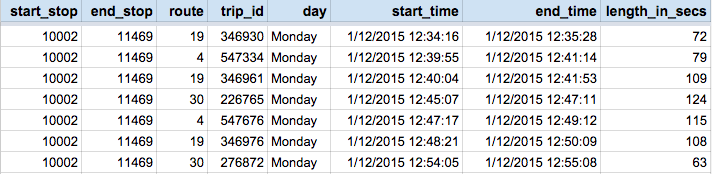
\includegraphics[width=0.7\textwidth]{figures/journey_time_10002.png}
\caption{\label{fig:journey_time_10002} List of journey time from stop 10002 to stop 11469}
\end{figure}

\par We then calculated the average journey time required to travel from 10002 to 11469 for each hour in each week of the day. This information is stored as a timetable, which would be used for further analysis.

\par Figure\ref{fig:timetable_10002} shows the timetable generated. Each cell indicates the average journey time required to travel from stop 10002 to stop 11469 at a give hour of a give week of day. The \textbf{NULL} values are due to a current databases performance issue. This will be resolved later.

\begin{figure}
\centering
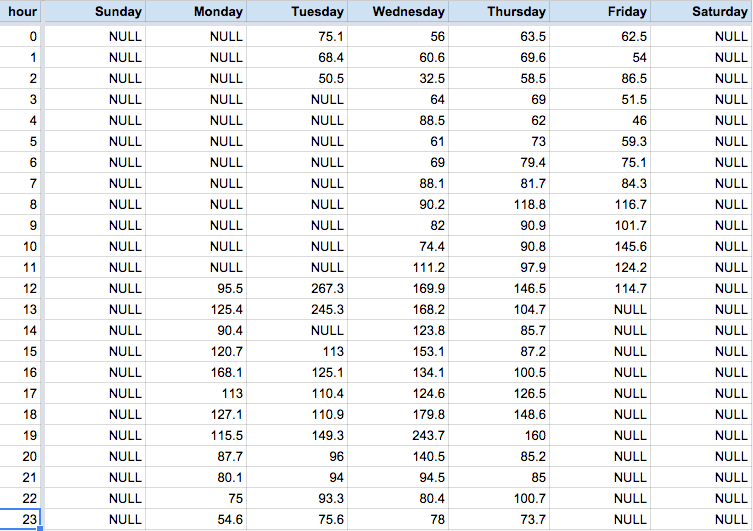
\includegraphics[width=0.9\textwidth]{figures/timetable_10002.png}
\caption{\label{fig:timetable_10002} Average journey time in seconds from stop 10002 to stop 11469 for each hour of each day of week}
\end{figure}

\par We plan to construct a timetable this way for each pair of the neighbouring bus stop.

\subsection{Negative Travel Time Filter}
\par In the travel\_time\_log generated, there were trips between two neighbouring stops with negative travel times, such as the entry shown in Table \ref{table:travel_time_log_negative}.

\begin{table}
\centering
\begin{tabular}{@{}lllllr@{}} \toprule
Start Stop & End Stop & Route & Start Time & End Time & Travel Time(sec) \\ \midrule
9326 & 15552 & W13 & 14:53:18 & 14:52:14 & -64 \\ \bottomrule
\end{tabular}
\caption{Travel Time Log Entry with Negative Travel Time}
\label{table:travel_time_log_negative}
\end{table}

\par This was because when we performed the join of the arrivals table, there was a more recent update on the arrival times for the start stop, whereas the arrival times of end stop had not been updated. In Table \ref{table:negative_travel_time_explained}, we observed that the Recorded Time for the end stop 9326 was more recent than that of the end stop. As a result, the arrival time for the end stop was earlier than the start stop, causing the travel time to be negative.

\begin{table}
\centering
\begin{tabular}{@{}lllllr@{}} \toprule
Stop Code & Route & Vehicle ID & Trip ID & Arrival Time & Recorded Time\\ \midrule
9326 & W13 & 18685 & 135229 &  14:53:18 & 14:48:25 \\ [0.4cm]
15552 & W13 & 18685 & 135229 & 14:52:14 & 14:44:02 \\ \bottomrule
\end{tabular}
\caption{Arrivals Entries to Explain Negative Travel Time}
\label{table:negative_travel_time_explained}
\end{table}

\par We filtered out these negative values before calculating the average travel time between neighbouring stops.
